% Style for a MSc paper at Warsaw School of Economics
% Michał Ramsza
% Fri Dec 22 14:49:36 CET 2023

% --- document class and other global stuff ---------------------------
\documentclass[english, twoside, 12pt, a4paper]{article}

% --- packages --------------------------------------------------------
\usepackage{textcomp}
\usepackage{times}
\usepackage{amsmath}
\usepackage{amsfonts}
\usepackage{amssymb}
\usepackage{amsthm}
\usepackage[T1]{fontenc}
\usepackage[utf8]{inputenc}
\usepackage{graphicx}
\usepackage{tikz}
\usepackage{xcolor}
\usepackage{enumitem}
\usepackage[english]{babel}
\usepackage{booktabs}
\usepackage{setspace}
\usepackage{csquotes}
\usepackage[centering, left=3.5cm, right=2.5cm, textheight=24cm]{geometry}

% --- packages for citations ------------------------------------------
\usepackage[backend=biber, style=authoryear, autocite=inline, defernumbers=true]{biblatex}
\addbibresource{refs.bib}

% --- package for automatic insertion of R code -----------------------
\usepackage{listings}
\lstset{%
   numbers=left,%
   tabsize=3,%
   numberstyle=\footnotesize,%
   basicstyle=\ttfamily \small \color{black},%
   keywordstyle=\ttfamily \small \color{black},%
   commentstyle=\ttfamily \small \color{gray},%
   stringstyle=\ttfamily \small \color{black},%
   identifierstyle=,%
   showstringspaces=false,%
   escapeinside={(*@}{@*)}}   
   
\lstset{
 literate={ą}{{\k a}}1
 {Ą}{{\k A}}1
 {ż}{{\. z}}1
 {Ż}{{\. Z}}1
 {ź}{{\' z}}1
 {Ź}{{\' Z}}1
 {ć}{{\' c}}1
 {Ć}{{\' C}}1
 {ę}{{\k e}}1
 {Ę}{{\k E}}1
 {ó}{{\' o}}1
 {Ó}{{\' O}}1
 {ń}{{\' n}}1
 {Ń}{{\' N}}1
 {ś}{{\' s}}1
 {Ś}{{\' S}}1
 {ł}{{\l}}1
 {Ł}{{\L}}1
}   

% --- support for links -----------------------------------------------	
\usepackage{hyperref}
\hypersetup{colorlinks=true,
            linkcolor=black,
            citecolor=darkgray,
            urlcolor=darkgray}
\usepackage{xurl}            
\urlstyle{same}

% --- support for large tables and other stuff ------------------------	
\usepackage{float}
\usepackage{caption}
\usepackage{subcaption}
\usepackage{wrapfig}

% --- support for game theory ------------------------------------------
\usepackage{sgame}

% --- support for no widows --------------------------------------------
\usepackage[defaultlines=4,all]{nowidow}

% -----------------------------------------------------------
\usepackage{setspace}

% --- definitions for environments -------------------------------------
\theoremstyle{definition}
    \newtheorem{condition}{Assumption}
    \newtheorem{example}{Example}      

\theoremstyle{plain}
    \newtheorem{definition}{Definition}    
    \newtheorem{proposition}{Proposition}
    \newtheorem{theorem}{Theorem}
    \newtheorem{cor}{Corollary}

\theoremstyle{remark}
    \newtheorem{remark}{Remark}

% --- other settings --------------------------------------------------
\linespread{1.5}
\frenchspacing
\sloppy
\allowdisplaybreaks[4]
\raggedbottom
\clubpenalty=10000
\widowpenalty=10000

% --- only if required ------------------------------------------------
\AtBeginDocument{\renewcommand*{\figurename}{Figure}}
\AtBeginDocument{\renewcommand*{\tablename}{Table}}

% --- changing definition of footnote ---------------------------------
\makeatletter
\renewcommand\footnotesize{%
   \@setfontsize\footnotesize\@ixpt{10}%
   \abovedisplayskip 8\p@ \@plus2\p@ \@minus4\p@
   \abovedisplayshortskip \z@ \@plus\p@
   \belowdisplayshortskip 4\p@ \@plus2\p@ \@minus2\p@
   \def\@listi{\leftmargin\leftmargini
               \topsep 4\p@ \@plus2\p@ \@minus2\p@
               \parsep 2\p@ \@plus\p@ \@minus\p@
               \itemsep \parsep}%
   \belowdisplayskip \abovedisplayskip
}
\makeatother

% --- useful definitions ----------------------------------------------
\newcommand{\code}[1]{\lstinline{#1}}

% ---------------------------------------------------------------------
\begin{document}

% --- strona tytulowa -------------------------------------------------
\begin{titlepage}
\centering


\includegraphics[width=0.66\textwidth]{logo.JPG}

\vspace*{0.5cm}
Master's study\\
\begin{flushleft}
Field of study: Advanced Analytics – Big Data\\
%Specjalność: <specjalność> % w przypadku braku należy pominać
%Forma studiów: <forma studiów (stacjonarne, itd.)>
\end{flushleft}

\vspace*{.5cm}
\rule{0cm}{1cm}\hfill
\begin{minipage}{9cm}
Author's first name and surname: Bogdan Bojarin\\
Student's register No.: 75184
\end{minipage}

\vspace*{1cm}
\begin{minipage}{12cm}
\centering
\Large
\textbf{Development of an intelligent system of document processing and generation based on machine learning methods}
\end{minipage}

\vspace*{2cm}
\rule{0cm}{1cm}\hfill
\begin{minipage}{9cm}
Master's thesis:\\
under the scientific supervision of:\\
dr hab. Michał Ramsza\\
written in\\
Institute of Mathematical Economics\\
\end{minipage}

\vfill
Warsaw 2025
\end{titlepage}

\rule{1ex}{0ex}\clearpage

% --- table of contents -----------------------------------------------
\cleardoublepage
\tableofcontents

% --- chapter ---------------------------------------------------------
\cleardoublepage
\section{Introduction}

This template is for the BSc/MSc papers at the Warsaw School of Economics. 

% --- chapter ---------------------------------------------------------
\clearpage
\section{Basic things}

\subsection{Compiling \LaTeX files}

The \verb+.tex+ file is just a plain text file. It contains the \LaTeX{} formatting codes together with the content of a paper. To get a \verb+.pdf+ file you have to compile the \verb+.tex+ file using a sequence \verb+pdflatex+, \verb+biblatex+, \verb+pdflatex+, \verb+pdflatex+. This sequence is a default in most editors designed for use with \LaTeX.

\subsection{Basic formatting for a text}

Paragraphs are coded by an empty line. That is is you want to start a new paragraph it is enough to leave an empty line and start typing like that:
\begin{verbatim}
This is the first paragraph.

This is the next paragraph.
\end{verbatim}

Everything about the paragraph is formatted for you including all indents and spacings. Again, you don't have to take care of it manually.

Basic text formatting, e.g. bold face and italic, is achieved with the following commands: \verb+\textbf{}+, \verb+\textit{}+, \verb+\underline{}+, producing \textbf{text}, \textit{text}, \underline{text}. I suggest not overusing those commands!

Alignment is done through environments \verb+center+, \verb+flushleft+ and \verb+\flushright+ giving the following examples.

\begin{center}
  This is centered.
\end{center}

\begin{flushleft}
  This is aligned to the left.
\end{flushleft}

\begin{flushright}
  This is aligned to the right. 
\end{flushright}

In other environments it is possible to use \verb+\centering+ to center content of that environment (like in \verb+figure+ or \verb+table+ environments).

\subsection{Fonts and fonts' sizes}

You do not change fonts and fonts' sizes! Technically it can be done but I will reject this.

% --- chapter ---------------------------------------------------------
\clearpage
\section{Mathematics}

This is testing footnotes\footnote{This is a footnote. We can put some math here \( x^2 - f(x) = g(x^2) \) which is not encouraged but sometimes necessary. The other thing we can do is to put here an URL \url{https://tex.stackexchange.com/questions/249415/set-font-size-for-footnotes}. }.

\subsection{Basic mathematics}

There are two types of mathematics inside a \LaTeX{} document. The first one is the in-line mathematics and the displayed mathematics. The first one looks like this: \( F(x) = \int_{-\infty}^{x} f(\omega) d\omega \) with the code looking like this: \verb!\( F(x) = \int_{-\infty}^{x} f(\omega) d\omega \)!. The displayed mathematics looks like that
\[
F(x) = \int_{-\infty}^{x} f(\omega) d\omega
\]
with the code
\begin{verbatim}
\[
F(x) = \int_{-\infty}^{x} f(\omega) d\omega
\]
\end{verbatim}
As you can see the same code is formatted differently depending on the type of mathematics.

\subsection{Referencing mathematics and other things}

To reference mathematics (only displayed formulas) you use the \verb+equation+ environment with a \verb+\label{}+ within. The reference is done through the \verb+\ref{}+ command. The example is
\begin{equation}
\label{eq:this-is-very-important-equation}
F(x) = \int_{-\infty}^{x} f(\omega) d\omega.
\end{equation}
To reference the equation you use the \verb+\ref{}+ command giving (\ref{eq:this-is-very-important-equation}). The \verb+\label{}+ / \verb+\ref{}+ pair works for anything that can be referenced.

\subsection{Some more mathematical formulas}

\LaTeX{} is known for producing beautifully typeset mathematical formulas. The above mathematical formulas are relatively simple. Here are slightly more complex formulas. Let \(A\) be a matrix
\[
A =
\left(
\begin{bmatrix}
1                   & \alpha^2       \\
2                   & \sqrt{\pi} - \log(x-\sin(y))
\end{bmatrix}^{2}
- 
\begin{bmatrix}
1                   & f(x)           \\
2                   & g(y)
\end{bmatrix}
\cdot
\begin{bmatrix}
x                                    \\
y
\end{bmatrix}
\right),
\]
where
\[
f(x) = 
\left\{
  \begin{aligned}
    \frac{1}{x}     & \quad \text{for \(x<-\frac{1}{2}\),} \\
    \frac{1}{1+x^2} & \quad \text{for \(x \geq -\frac{1}{2}\)}
  \end{aligned}
\right.
\]
and
\[
g(y) = \sin\left(\frac{\mathrm{\mathbf{E}}(X)}{\cos(y) + \log(y)}\right), 
\quad\text{where \( X \sim \mathrm{N}(0, \sigma)  \).}
\]
Note that the above formulas are parts of a sentence. Thus, you still use proper punctuation. In \LaTeX{}, we can also typeset diagrams of arbitrary complexity. However, this requires another language for defining graphical scenes: TikZ (\url{https://tikz.org/}). 

\begin{figure}[hbt]
  \centering

\resizebox{0.6\textwidth}{!}{%
\usetikzlibrary {arrows.meta,automata,positioning,shadows}
\begin{tikzpicture}[->,>={Stealth[round]},shorten >=1pt,auto,node distance=2.8cm,on grid,semithick,
                    every state/.style={fill=red,draw=none,circular drop shadow,text=white}]

  \node[initial,state] (A)                    {$q_a$};
  \node[state]         (B) [above right=of A] {$q_b$};
  \node[state]         (D) [below right=of A] {$q_d$};
  \node[state]         (C) [below right=of B] {$q_c$};
  \node[state]         (E) [below=of D]       {$q_e$};

  \path (A) edge              node {0,1,L} (B)
            edge              node {1,1,R} (C)
        (B) edge [loop above] node {1,1,L} (B)
            edge              node {0,1,L} (C)
        (C) edge              node {0,1,L} (D)
            edge [bend left]  node {1,0,R} (E)
        (D) edge [loop below] node {1,1,R} (D)
            edge              node {0,1,R} (A)
        (E) edge [bend left]  node {1,0,R} (A);

   \node [right=3cm,text width=7cm] at (C)
   { \small
     The current candidate for the busy beaver for five states. It is
     presumed that this Turing machine writes a maximum number of
     $1$'s before halting among all Turing machines with five states
     and the tape alphabet $\{0, 1\}$. Proving this conjecture is an
     open research problem.
   };
\end{tikzpicture}
}

  \captionsetup{margin=10pt,font=small,labelfont=bf,width=.8\textwidth}

  \caption[Example of a diagram]{This is a simple diagram of a Turing machine. With TikZ, we can prepare diagrams of any complexity. \textit{Source:} \url{https://tikz.org/}.}\label{fig:diagram}
\end{figure}

For those of you doing game theory, the TikZ is a great solution for visualizing extensive-form games. For normal-form games, we have a  simpler solution. It is very easy to typeset a normal-form game. Below is an example of such a game. 

\begin{center}

\begin{game}{3}{3}
    & $L$    & $M$    & $H$    \\
$L$ & $16,9$ & $3,13$ & $0,3$  \\
$M$ & $21,1$ & $10,4$ & $-1,0$ \\
$H$ & $9,0$  & $5,-4$ & $-5,-15$
\end{game}
 
\end{center}

% --- chapter ---------------------------------------------------------
\clearpage
\section{Figures and tables}

Both figures and tables use the same ideas. To insert a table, you use the \verb+table+ environment. The following tables are just examples of what can be automatically generated with the R and Python programming languages.

\begin{table}[hbt]
  \centering

  \captionsetup{margin=10pt,font=small,labelfont=bf,width=.8\textwidth}

  \caption[Short name for a table]{This is an example of a table generated in the R programming language. The script generating the table is \code{example.R}.}
  \label{tab:exceptional-table}

  \vspace*{2ex}
  \footnotesize

  
% Table created by stargazer v.5.2.3 by Marek Hlavac, Social Policy Institute. E-mail: marek.hlavac at gmail.com
% Date and time: ptk, gru 22, 2023 - 16:48:02
\begin{tabular}{@{\extracolsep{5pt}} cccc} 
\\[-1.8ex]\hline 
\hline \\[-1.8ex] 
 & Values x & Values y & Class \\ 
\hline \\[-1.8ex] 
1 & -0.12 & 0.73 & Down \\ 
2 & -1.54 & -2 & Up \\ 
3 & -0.64 & -0.36 & Down \\ 
4 & -0.96 & -0.43 & Up \\ 
5 & 0.92 & 1.72 & Down \\ 
\hline \\[-1.8ex] 
\end{tabular} 

  
\end{table}

\begin{table}[hbt]
  \centering

  \captionsetup{margin=10pt,font=small,labelfont=bf,width=.8\textwidth}

  \caption[Short name for a table]{This is another example of a table generated in the R programming language. This table is automatically generated from the linear regression model. }
  \label{tab:lm}

  \vspace*{2ex}
  \footnotesize

  
% Table created by stargazer v.5.2.3 by Marek Hlavac, Social Policy Institute. E-mail: marek.hlavac at gmail.com
% Date and time: ptk, gru 22, 2023 - 16:55:58
\begin{tabular}{@{\extracolsep{5pt}}lc} 
\\[-1.8ex]\hline 
\hline \\[-1.8ex] 
 & \multicolumn{1}{c}{\textit{Dependent variable:}} \\ 
\cline{2-2} 
\\[-1.8ex] & y \\ 
\hline \\[-1.8ex] 
 x & 1.989$^{***}$ \\ 
  & (0.032) \\ 
  & \\ 
 Constant & 1.020$^{***}$ \\ 
  & (0.033) \\ 
  & \\ 
\hline \\[-1.8ex] 
Observations & 1,000 \\ 
R$^{2}$ & 0.796 \\ 
Adjusted R$^{2}$ & 0.796 \\ 
Residual Std. Error & 1.029 (df = 998) \\ 
F Statistic & 3,903.749$^{***}$ (df = 1; 998) \\ 
\hline 
\hline \\[-1.8ex] 
\textit{Note:}  & \multicolumn{1}{r}{$^{*}$p$<$0.1; $^{**}$p$<$0.05; $^{***}$p$<$0.01} \\ 
\end{tabular} 

  
\end{table}

To insert a figure, you need to have a figure. In the \code{./figs} directory, there are figures generated with the R and Python scripts, and the following is an example of the \verb+figure+ environment. Figure~\ref{fig:xxx} is slightly more complex than just a simple figure, but it is useful to have such a template. It is possible to reference subfigures as \ref{fig:xxxa} and \ref{fig:xxxb}.

\begin{figure}[hbt]
  \centering

  \begin{subfigure}[t]{0.45\textwidth}
    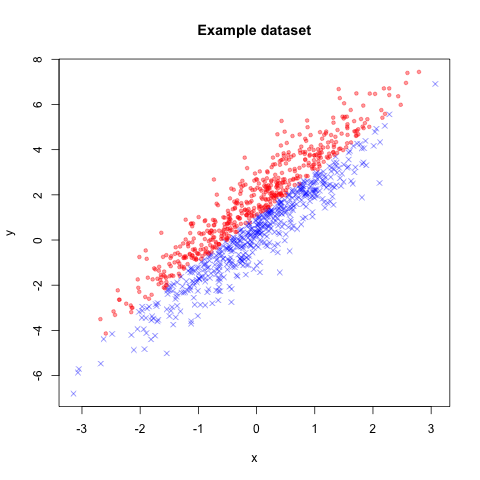
\includegraphics[width=\textwidth]{./figs/fig_00.png}
  \end{subfigure}

  \captionsetup{margin=10pt,font=small,labelfont=bf,width=.8\textwidth}

  \caption[Short name]{This is an example figure generated in the R programming language.  \textit{Source:} own calculations.}\label{fig:xxx1}
\end{figure}

\begin{figure}[hbt]
  \centering
  \begin{subfigure}[t]{0.45\textwidth}
    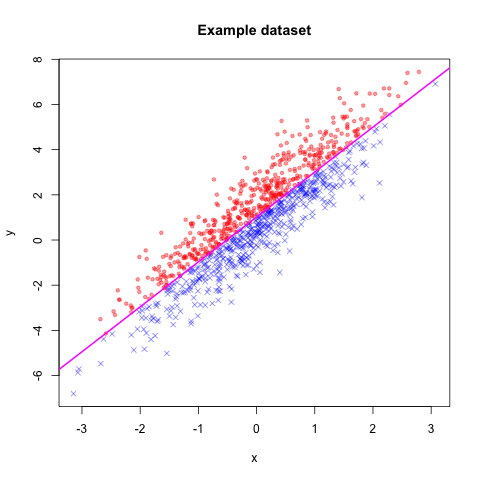
\includegraphics[width=\textwidth]{./figs/fig_01.png}
    \caption{This is another visualization done in the R programming language in the script \code{example.R}. This caption is wrapped at the right width, and the height is being compensated.}
    \label{fig:xxxa}
  \end{subfigure}
  \hfill
  \begin{subfigure}[t]{0.45\textwidth}
    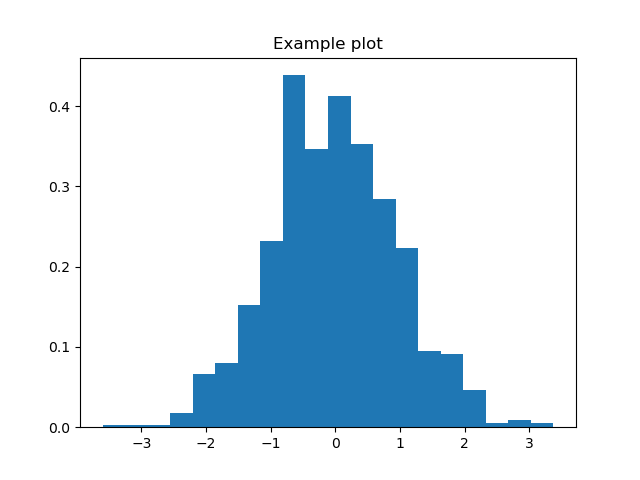
\includegraphics[width=\textwidth]{./figs/fig_02.png}
    \caption{This figure was generated in the Python programming language. The script \code{example.py} creates this figure and the additional table.}
    \label{fig:xxxb}
  \end{subfigure}
  
  \captionsetup{margin=10pt,font=small,labelfont=bf,width=.8\textwidth}

  \caption[Short caption 2]{This is the main caption and it is below the figures. Both figures were automatically created in scripts. If we want to change the figure, we change the script only. \textit{Source:} own calculations}\label{fig:xxx}
\end{figure}


\begin{table}[hbt]
  \centering

  \captionsetup{margin=10pt,font=small,labelfont=bf,width=.8\textwidth}

  \caption[Pandas table]{This is another table generated by the Python script \code{example.py}. This table looks a little bit different, but it's acceptable.}
  \label{tab:pandasdf}

  \vspace*{2ex}
  \footnotesize

  \begin{tabular}{lr}
\toprule
Class & Values \\
\midrule
j & 0.953570 \\
M & 0.183956 \\
X & 1.243109 \\
I & -1.032789 \\
N & 0.443236 \\
K & -1.602915 \\
l & -1.273745 \\
l & 2.209001 \\
r & 0.190158 \\
R & 0.873841 \\
\bottomrule
\end{tabular}

  
\end{table}


% --- chapter ---------------------------------------------------------
\clearpage
\section{Bibliography}

\begin{wrapfigure}{r}{.5\textwidth}
\centering

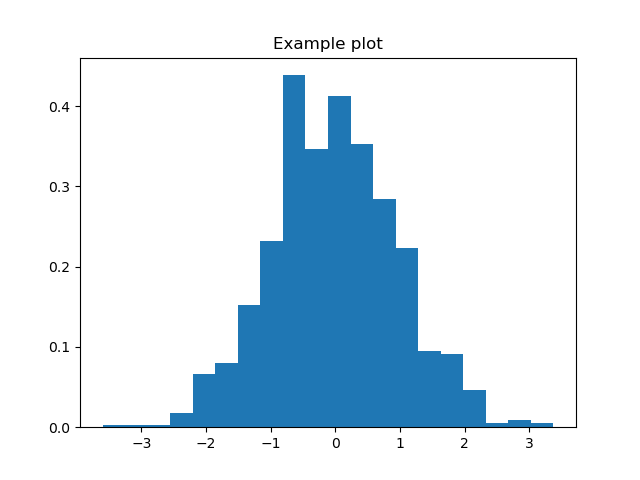
\includegraphics[width=.4\textwidth]{./figs/fig_02.png}

\captionsetup{margin=10pt,font=small,labelfont=bf,width=.42\textwidth}

  \caption[Short caption 2]{This is how one can wrap a text around a figure. \textit{Source:} own calculations}\label{fig:yyy}


\end{wrapfigure}

The content for the bibliography is in a different file named \verb+refs.bib+. You can change the name but then you have to change the information in this file from \verb+\bibliography{refs}+ to \verb+\bibliography{new-name}+ where \verb+new-name+ is the name of your file. The file \verb+refs.bib+ contains some examples for books and papers.

The process of citation is simple. The command  \verb+\textcite{garland2010}+ gives this \textcite{garland2010} and puts all information into the bibliography section at the end. Everything is sorted and formatted, so you don't have to worry about this. An example of a paper with many authors is \cite{benaim2003} or \cite{osborne1998}. We can cite online resources \cite{bbb} or \cite{cnn}. We can use the following citation \parencite{benaim2003} or like this \footcite{benaim2003} or like this \footfullcite{cnn}.

% --- appendices ------------------------------------------------------
\appendix

% ---------------------------------------------------------------------
\clearpage
\section{Appendix: Some important stuff}

This is an appendix. This is the place to put it if you have some additional figures, tables, or a code. The really long tables or really wide tables should be placed in additional files e.g., XLSX. 

\lstinputlisting[firstline=51,lastline=60,basicstyle=\ttfamily \footnotesize \color{black}]{../code_r/example.R}

Below, there is a fragment of the \code{example.py} script that creates a Pandas tabel and exports to \LaTeX{}.

\lstinputlisting[firstline=16,lastline=29,basicstyle=\ttfamily \footnotesize \color{black}]{../code_python/example.py}

% --- bibliography ----------------------------------------------------
\clearpage
\printbibliography[heading=subbibliography,nottype=online,title={References}]
\printbibliography[heading=subbibliography,type=online,title={Online references}]


% --- abstract --------------------------------------------------------
\clearpage
\addcontentsline{toc}{section}{List of tables}
\listoftables

% --- abstract --------------------------------------------------------
\clearpage
\addcontentsline{toc}{section}{List of figures}
\listoffigures



% --- abstract --------------------------------------------------------
\clearpage
\addcontentsline{toc}{section}{Streszczenie}
\section*{Streszczenie}

Tutaj zamieszczają Państwo streszczenie pracy. Streszczenie powinno być długości około pół strony.


\end{document}


%%% Local Variables:
%%% mode: latex
%%% TeX-master: t
%%% End:
